\documentclass[conference]{IEEEtran}
\usepackage[utf8]{inputenc}
\usepackage[T1]{fontenc}
\usepackage[spanish,es-noshorthands,es-tabla]{babel}
\usepackage{graphicx}
\usepackage{booktabs}
\usepackage{array}
\usepackage{amsmath,amssymb}
\usepackage{url}
\usepackage[hidelinks]{hyperref}
\graphicspath{{figuras/}}
\newcolumntype{L}[1]{>{\raggedright\arraybackslash}p{#1}}
% \input no es expandible y rompe \bottomrule dentro de tabular; el primitivo sí funciona.
\makeatletter\newcommand{\tabla}[1]{\@@input tablas/#1.tex }\makeatother

\begin{document}

\title{Predicción de cancelación de reservaciones de hoteles con aprendizaje supervisado\\
\large Segundo entregable: preparación de los datos y modelado}

\author{\IEEEauthorblockN{Humberto Ángel Plata Durán (0250945) y Diego Hernández Ortiz (0255531)}
\IEEEauthorblockA{Aprendizaje de Máquina, Universidad Panamericana, Ciudad de México\\
Docente: Dra. Antonieta Teodora Martínez Velasco\\
Otoño 2026, 18 de noviembre}}

\maketitle

% La numeración continúa la de la Entrega 1 (7 figuras y 5 tablas).
\setcounter{figure}{7}
\setcounter{table}{5}

\begin{abstract}
En esta entrega implementamos las fases 3 y 4 de CRISP-DM sobre las 119,390 reservaciones de la
Entrega 1. La preparación aplica las decisiones de la Tabla V: elimina 180 registros imposibles y
las variables con fuga, convierte los nulos con significado en categorías, crea 14 variables nuevas
y parte los datos por fecha de llegada. Todo lo que aprende de los datos (medianas, percentiles,
escalas, categorías frecuentes y la frecuencia de cada agencia) vive en un \texttt{Pipeline}
ajustado solo con entrenamiento. Comparamos una regresión logística que programamos desde cero
con NumPy, un bosque aleatorio y un \emph{gradient boosting}, con validación cruzada agrupada por
duplicados y búsqueda de hiperparámetros. El modelo final (\emph{gradient boosting}) llega a una
PR-AUC de 0.873 en validación y de 0.784 en la prueba temporal (mayo a agosto de 2017). La caída
se explica por un aumento de las cancelaciones del resort en 2017. Con un umbral elegido por
costo esperado, el modelo anticipa el 45\,\% del ingreso en riesgo del periodo de prueba con 81\,\%
de precisión. Las variables sospechosas de fuga habrían subido la PR-AUC 5.3 puntos, por lo que
las dejamos fuera.
\end{abstract}

\begin{IEEEkeywords}
cancelación de reservaciones, clasificación supervisada, regresión logística, gradient boosting,
fuga de información, SHAP, CRISP-DM
\end{IEEEkeywords}

\section{Introducción}

En la Entrega 1 planteamos el problema como una clasificación binaria supervisada sobre el conjunto
\emph{Hotel Booking Demand}~\cite{antonio2019,tidytuesday}: estimar, con la información disponible
el día anterior a la llegada, la probabilidad de que una reservación se cancele, como proponen
Antonio \emph{et al.}~\cite{antonio2017}. Del análisis exploratorio salieron cuatro decisiones que guían esta entrega: medir con
PR-AUC y no con exactitud, excluir tres variables con fuga confirmada~\cite{kaufman} y medir el efecto de otras
tres sospechosas, validar de forma temporal y agrupada por los duplicados, y esperar que la señal
venga del canal, el depósito, la anticipación y el historial del cliente.

Este documento cubre las fases 3 y 4 de CRISP-DM~\cite{chapman}: la preparación de los datos (Sección~\ref{sec:prep}) y el modelado
(Sección~\ref{sec:modelo}), evalúa una sola vez en la prueba temporal
(Sección~\ref{sec:prueba}) y adelanta el despliegue del modelo como servidor MCP
(Sección~\ref{sec:despliegue}). La Sección~\ref{sec:objetivos} revisa los objetivos OE1 a OE5. El
código, los cuadernos y el modelo están en el repositorio del proyecto~\cite{repo}.

\section{Preparación de los datos}\label{sec:prep}

Separamos el código en dos partes. Lo que no aprende nada de los datos (reglas fila por fila de
limpieza e ingeniería de características) se aplica antes de partir y no puede filtrar
información. Lo que sí aprende parámetros va dentro de un \texttt{Pipeline} de
scikit-learn~\cite{pedregosa} que se ajusta solo con el conjunto de entrenamiento y se vuelve a
ajustar en cada pliegue de la validación cruzada. Las mismas funciones se usan en el servidor que
sirve el modelo, así que entrenamiento y operación ven exactamente las mismas transformaciones.

\subsection{Limpieza}

La Tabla~\ref{tab:limpieza} resume los tratamientos. Solo eliminamos las 180 reservaciones con
cero huéspedes (0.15\,\% de los datos). Los nulos de \texttt{agent}, \texttt{company} y
\texttt{country} se vuelven categorías propias, como acordamos en la Entrega 1, y el plan de
comidas \emph{Undefined} se recodifica como \texttt{SC}, porque las dos etiquetas significan
``sin plan''. Quitamos \texttt{reservation\_status}, \texttt{reservation\_status\_date},
\texttt{assigned\_room\_type} y \texttt{arrival\_date\_year}.

Los duplicados no se borran. A cada fila le asignamos una firma de grupo (filas idénticas en las
32 columnas originales comparten firma): quedan 87,230 grupos, y 40,141 filas pertenecen a un grupo
de más de una. La validación cruzada usa esa firma para que dos copias nunca queden una en
entrenamiento y otra en validación.

\begin{table*}[t]
\centering
\caption{Tratamientos de limpieza}\label{tab:limpieza}
\begin{tabular}{L{4.2cm}L{9.5cm}r}
\toprule
Problema & Tratamiento & Filas \\
\midrule
\tabla{limpieza}
\bottomrule
\end{tabular}
\end{table*}

\subsection{Ingeniería de características}

Creamos 14 variables (Tabla~\ref{tab:variables}). La fecha de llegada, que en el archivo viene
partida en año, mes y día, da el día de la semana y un ángulo de temporada (seno y coseno del mes,
para que diciembre y enero queden cerca). El historial del cliente se resume en una tasa de
cancelación previa, y el canal en banderas de agencia y empresa. La frecuencia histórica de la
agencia, que prometimos en la Entrega 1, es la única que aprende de los datos: es la proporción de
reservaciones de entrenamiento que hizo cada agencia, así que se calcula dentro del
\texttt{Pipeline}.

\begin{table}[t]
\centering
\caption{Variables derivadas}\label{tab:variables}
\begin{tabular}{L{3.3cm}L{4.6cm}}
\toprule
Variable & Construcción \\
\midrule
\texttt{noches}, \texttt{huespedes} & suma de noches; adultos + niños + bebés \\
\texttt{estancia\_cero} & 0 noches (\emph{day-use}) \\
\texttt{proporcion\_fin\_semana} & noches de fin de semana / noches \\
\texttt{tiene\_ninos} & niños + bebés $>$ 0 \\
\texttt{mes\_sin}, \texttt{mes\_cos} & mes de llegada como ángulo \\
\texttt{dia\_semana}, \texttt{llegada\_fin\_semana} & día de la semana de la llegada \\
\texttt{tiene\_agente}, \texttt{tiene\_empresa} & \texttt{agent} o \texttt{company} presentes \\
\texttt{historial\_reservas} & reservas previas canceladas + no canceladas \\
\texttt{tasa\_cancelacion\_previa} & cancelaciones previas / historial \\
\texttt{adr\_por\_persona} & ADR / huéspedes \\
\texttt{frecuencia\_agente} & proporción de reservas de la agencia (aprendida) \\
\bottomrule
\end{tabular}
\end{table}

La Fig.~\ref{fig:variables} muestra las que más separan. Los clientes con historial sin
cancelaciones casi nunca cancelan (2\,\%), y los que ya cancelaron antes lo vuelven a hacer el
92\,\% de las veces. Con agencia la tasa es de 39\,\% y sin agencia de 25\,\%; con empresa baja a
17\,\%, y las estancias de cero noches cancelan apenas 3.6\,\%. El día de la semana y el precio por
persona aportan poco por sí solos, pero no tienen una relación monótona con el objetivo y los
árboles pueden aprovecharlos. Lo mismo pasa con la frecuencia de la agencia: su correlación con la
cancelación es casi nula ($\rho = 0.005$), aunque el quintil intermedio, formado sobre todo por las
agencias 240 y 1, cancela 47.5\,\%, contra 31--37\,\% del resto.

\begin{figure*}[t]
\centering
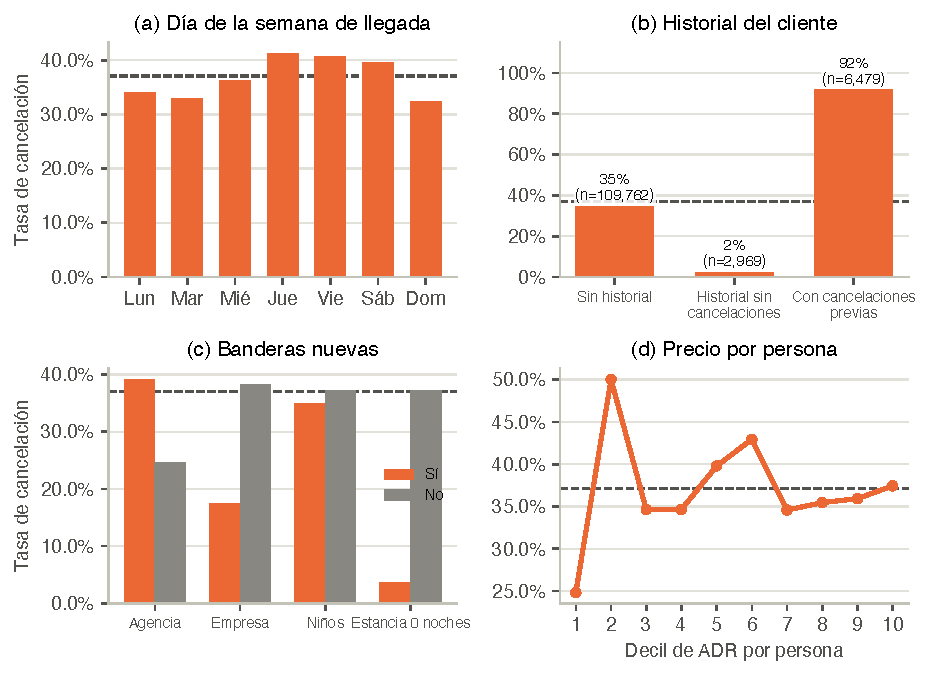
\includegraphics[width=0.78\textwidth]{fig8_variables_nuevas.pdf}
\caption{Tasa de cancelación según las variables nuevas: día de llegada (a), historial del cliente
(b), banderas de canal y estancia (c) y decil de ADR por persona (d). La línea punteada es la tasa
global.}\label{fig:variables}
\end{figure*}

\subsection{Partición temporal}

Como la tasa de cancelación cambia con el tiempo, reservamos las llegadas a partir del 1 de mayo
de 2017 como prueba (Tabla~\ref{tab:particion}, Fig.~\ref{fig:particion}). Es el uso real del
modelo: aprender del pasado y predecir llegadas futuras. Ningún grupo de duplicados queda partido
entre los dos conjuntos, porque las copias idénticas comparten fecha de llegada. La tasa de
cancelación de la prueba (40.6\,\%) es mayor que la del entrenamiento (36.3\,\%), y el salto viene
casi todo del resort: de 26.0\,\% a 36.2\,\%.

\begin{table*}[t]
\centering
\caption{Partición temporal}\label{tab:particion}
\begin{tabular}{llrrrrr}
\toprule
Conjunto & Llegadas & Reservas & \% total & Tasa & Tasa urbano & Tasa resort \\
\midrule
\tabla{particion}
\bottomrule
\end{tabular}
\end{table*}

\begin{figure}[t]
\centering
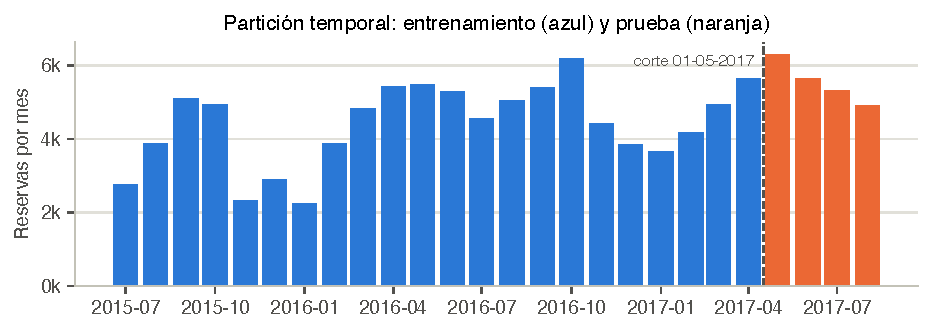
\includegraphics[width=\columnwidth]{fig9_particion.pdf}
\caption{Reservaciones por mes de llegada: entrenamiento (azul) y prueba (naranja).}\label{fig:particion}
\end{figure}

\subsection{Transformación}

El \texttt{Pipeline} encadena cinco pasos ajustados solo con entrenamiento: recorte del ADR y del
ADR por persona al percentil 99.9 (300 y 195; el ADR de 5,400 desaparece y el negativo pasa a
cero), frecuencia de la agencia, imputación con la mediana (los 4 nulos de \texttt{children}),
transformación y codificación. Para la regresión logística los conteos con cola larga pasan por
$\log(1+x)$ y todas las numéricas se estandarizan, porque el descenso por gradiente es inestable
cuando las escalas difieren mucho (Fig.~\ref{fig:transformacion}). Los árboles reciben las
variables sin escalar: sus particiones no cambian con transformaciones monótonas. El
\emph{one-hot} agrupa en una sola columna las categorías con menos de 1\,\% de las filas, como
indica la Tabla V; de 316 agencias quedan 14 columnas y de 330 empresas, 2. Las 38 variables de
entrada terminan en 81 columnas numéricas sin nulos. Una categoría que no se vio en entrenamiento
cae en la columna de infrecuentes, y una agencia nueva recibe frecuencia cero.

\begin{figure}[t]
\centering
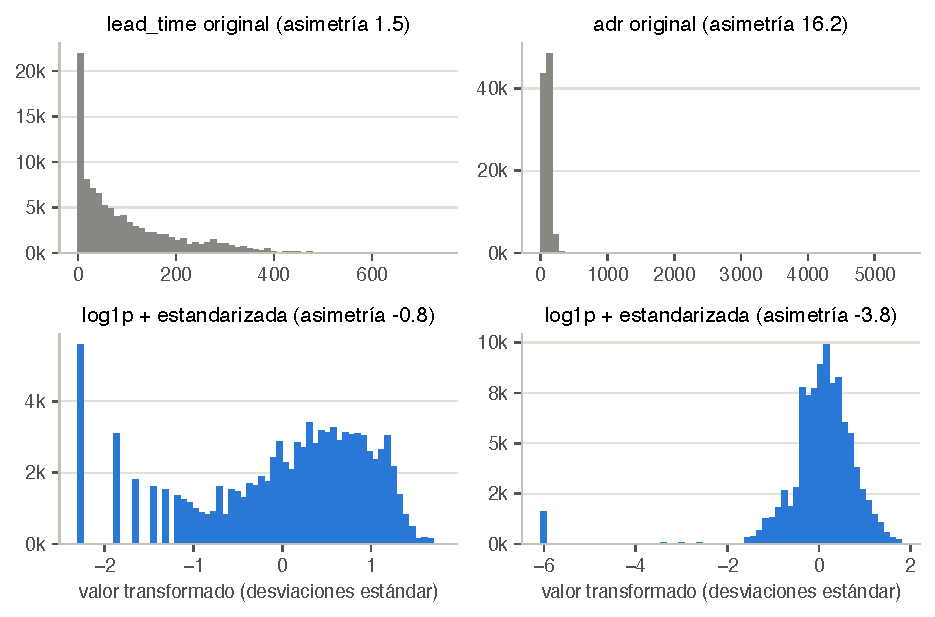
\includegraphics[width=\columnwidth]{fig10_transformacion.pdf}
\caption{\texttt{lead\_time} y \texttt{adr} antes (gris) y después (azul) de $\log(1+x)$ y
estandarización.}\label{fig:transformacion}
\end{figure}

\section{Modelado}\label{sec:modelo}

\subsection{Tipo de problema y protocolo}

La variable objetivo es binaria y está etiquetada, así que se trata de clasificación supervisada;
no es regresión ni \emph{clustering}. Nos interesa además la probabilidad, para ordenar las
reservaciones por riesgo. La métrica principal es la PR-AUC~\cite{saito}, y reportamos también
ROC-AUC, F1, \emph{recall} y precisión. Validamos con \texttt{StratifiedGroupKFold} de 5 pliegues
sobre el entrenamiento, estratificando por la clase y agrupando por la firma de duplicado. Los tres
modelos usan pesos de clase balanceados. La prueba temporal se usa una sola vez, al final.

\subsection{Regresión logística desde cero}

Programamos el modelo base solo con NumPy para entender qué ocurre dentro del entrenamiento. Para
una reservación con variables $x$, el modelo calcula
\begin{equation}
\hat p = \sigma(w^\top x + b) = \frac{1}{1 + e^{-(w^\top x + b)}},
\end{equation}
y minimiza la entropía cruzada ponderada con penalización L2,
\begin{equation}
L = -\frac{1}{\sum_i s_i}\sum_i s_i\big[y_i \log \hat p_i + (1-y_i)\log(1-\hat p_i)\big]
+ \frac{\lambda}{2}\lVert w\rVert^2,
\end{equation}
donde $s_i = n/(2n_{y_i})$ le da más peso a la clase minoritaria. Como
$\sigma'(z) = \sigma(z)(1-\sigma(z))$, el gradiente queda en una forma compacta:
\begin{equation}
\nabla_w L = \frac{1}{\sum_i s_i} X^\top\big[s \odot (\hat p - y)\big] + \lambda w .
\end{equation}
El entrenamiento es descenso por gradiente con mini-lotes de 1,024 reservaciones, barajando en
cada época, y se detiene cuando la pérdida deja de bajar durante 5 épocas. Implementamos también
una sigmoide numéricamente estable y la interfaz \texttt{fit}/\texttt{predict\_proba} para poder
usar la clase dentro del \texttt{Pipeline} y de la validación cruzada.

Antes de entrenar comparamos el gradiente analítico con uno numérico por diferencias centrales: el
error relativo fue menor a $10^{-7}$. Después lo comparamos con \texttt{LogisticRegression} de
scikit-learn, que minimiza la misma función con L-BFGS. La versión NumPy converge en 44 épocas y
llega casi al mismo resultado en entrenamiento (ROC-AUC 0.863 contra 0.864), con coeficientes que
correlacionan 0.92 (Fig.~\ref{fig:numpy}). No son idénticos porque el descenso con tasa fija se
detiene cerca del mínimo, y porque el \emph{one-hot} con intercepto deja direcciones redundantes
que una penalización tan pequeña apenas fija.

\begin{figure}[t]
\centering
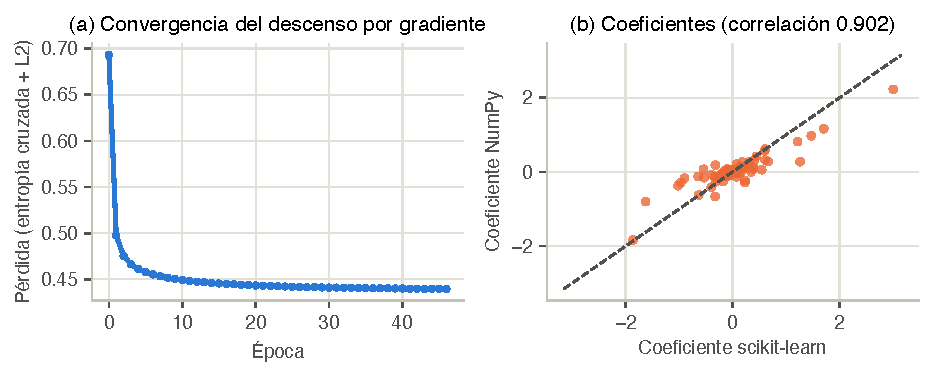
\includegraphics[width=\columnwidth]{fig11_logistica_numpy.pdf}
\caption{Regresión logística con NumPy: pérdida por época (a) y coeficientes contra los de
scikit-learn (b).}\label{fig:numpy}
\end{figure}

\subsection{Modelos de árboles}

Comparamos la logística con dos ensambles. El bosque aleatorio~\cite{breiman} promedia árboles
profundos entrenados con \emph{bootstrap} y un subconjunto de variables en cada división. El
\emph{gradient boosting}~\cite{friedman} construye árboles en secuencia, cada uno corrigiendo el
error de los anteriores; usamos \texttt{HistGradientBoostingClassifier}, que discretiza las
variables en histogramas como LightGBM~\cite{lightgbm} y entrena rápido con 97 mil filas.

\subsection{Ajuste de hiperparámetros}

Para la logística probamos una rejilla de 12 combinaciones de tasa de aprendizaje $\eta$ y
regularización $\lambda$. Para el \emph{gradient boosting} hicimos una búsqueda aleatoria de 20
combinaciones~\cite{bergstra} sobre la tasa de aprendizaje, las hojas por árbol, el mínimo de
reservaciones por hoja, la regularización L2 y la fracción de variables, con parada temprana. El
bosque, que es el más costoso, tuvo 6 combinaciones. Cada combinación se evaluó con los mismos 5
pliegues (Tabla~\ref{tab:cv}, Tabla~\ref{tab:hiper}, Fig.~\ref{fig:hiper}).

\begin{table*}[t]
\centering
\caption{Validación cruzada agrupada (5 pliegues, escenario sin variables sospechosas)}\label{tab:cv}
\begin{tabular}{lcccccc}
\toprule
Modelo & PR-AUC (por defecto) & PR-AUC (ajustado) & ROC-AUC & F1 & Recall & Precisión \\
\midrule
\tabla{modelos_cv}
\bottomrule
\end{tabular}
\end{table*}

\begin{table*}[t]
\centering
\caption{Mejores hiperparámetros}\label{tab:hiper}
\begin{tabular}{lL{12.5cm}}
\toprule
Modelo & Hiperparámetros \\
\midrule
\tabla{hiperparametros}
\bottomrule
\end{tabular}
\end{table*}

\begin{figure}[t]
\centering
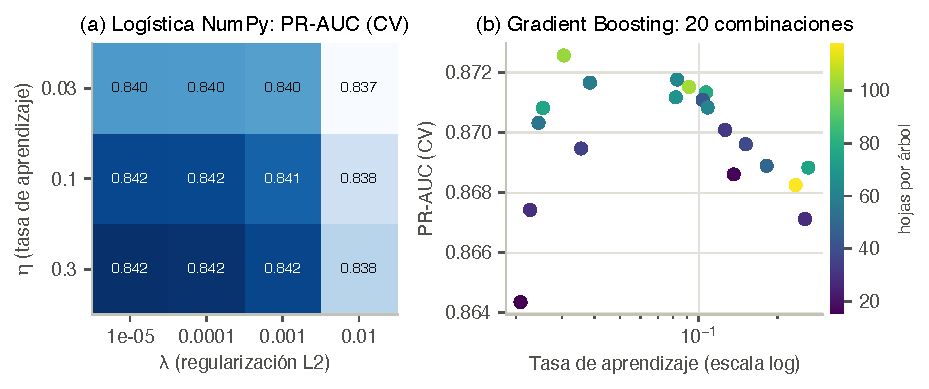
\includegraphics[width=\columnwidth]{fig12_hiperparametros.pdf}
\caption{PR-AUC en validación para la rejilla de la logística (a) y para la búsqueda aleatoria del
\emph{gradient boosting} (b).}\label{fig:hiper}
\end{figure}

Los árboles superan a la logística por unos 3 puntos de PR-AUC (0.873 contra 0.842), una diferencia
tres veces mayor que la desviación entre pliegues. Era lo que esperábamos por la Entrega 1: la
señal está repartida y no es lineal. La logística prefiere la regularización más débil y casi no
mejora con el ajuste; le falta capacidad, no le sobra varianza. El \emph{gradient boosting} es el
que más gana (de 0.867 a 0.873) y empata con el bosque. Lo elegimos como modelo final porque tiene
mayor \emph{recall} y porque pesa 3~MB, contra cientos de megabytes de un bosque profundo, lo que
importa para el despliegue.

\subsection{Escenario con variables sospechosas}

Con los mismos hiperparámetros, agregar \texttt{country}, \texttt{required\_car\_parking\_spaces}
y \texttt{booking\_changes} sube la PR-AUC de validación de 0.873 a 0.926 y el \emph{recall} en casi
10 puntos. Es demasiado para tres variables, y coincide con lo que sospechábamos: el
estacionamiento y el país se capturan o corrigen al llegar el huésped, y los cambios se cuentan
hasta el \emph{check-in}. El día anterior a la llegada esos valores no existen o no son
definitivos, así que el modelo final se queda en el escenario conservador y el otro sirve solo
como cota superior.

\subsection{Umbral de decisión según costos}

El OE4 pide un umbral basado en lo que cuesta cada error. La acción que dispara una predicción
positiva es sobrevender la habitación. Un falso negativo deja el cuarto vacío y cuesta el ingreso
de la reservación (ADR por noches); un falso positivo obliga a reubicar a un huésped que sí llegó.
Suponemos que reubicar cuesta $\kappa = 1.5$ veces el ingreso (cuarto en otro hotel, traslado y
compensación) y buscamos el umbral que minimiza el costo total sobre las predicciones fuera de
pliegue del entrenamiento~\cite{elkan}. Con probabilidades calibradas el umbral sería
$\kappa/(1+\kappa) = 0.6$, pero los pesos balanceados las desplazan, así que lo buscamos de forma
empírica.

El umbral óptimo es 0.72, más alto que el que maximiza F1 (0.50): si equivocarse al sobrevender
cuesta más, conviene hacerlo solo cuando el modelo está muy seguro. Con ese umbral el costo
esperado baja 47\,\% respecto a no usar el modelo. La Tabla~\ref{tab:umbral} y la
Fig.~\ref{fig:umbral} muestran que la decisión depende del supuesto: $\kappa$ tiene que fijarlo el
hotel con sus costos reales.

\begin{table}[t]
\centering
\caption{Umbral óptimo según el costo relativo de reubicar ($\kappa$)}\label{tab:umbral}
\begin{tabular}{ccccc}
\toprule
$\kappa$ & Umbral & Recall & Precisión & Ahorro \\
\midrule
\tabla{umbral}
\bottomrule
\end{tabular}
\end{table}

\begin{figure}[t]
\centering
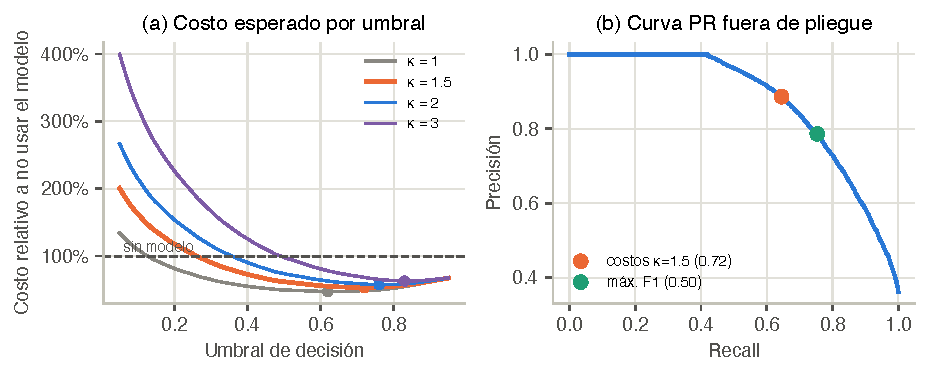
\includegraphics[width=\columnwidth]{fig15_umbral_costos.pdf}
\caption{Costo esperado relativo a no usar el modelo según el umbral (a) y umbrales sobre la curva
precisión-\emph{recall} fuera de pliegue (b).}\label{fig:umbral}
\end{figure}

\section{Evaluación en la prueba temporal}\label{sec:prueba}

La Tabla~\ref{tab:prueba} y la Fig.~\ref{fig:prueba} resumen la única evaluación en las llegadas
de mayo a agosto de 2017. El modelo final obtiene PR-AUC de 0.784 y ROC-AUC de 0.816. Cumple la
meta de PR-AUC del OE4 (0.75), pero no la de ROC-AUC (0.85).

\begin{table*}[t]
\centering
\caption{Desempeño en la prueba temporal (umbral 0.72 para el modelo final; 0.5 para los demás)}\label{tab:prueba}
\begin{tabular}{lcccccc}
\toprule
Modelo & PR-AUC & ROC-AUC & F1 & Recall & Precisión & Exactitud \\
\midrule
\tabla{prueba}
\bottomrule
\end{tabular}
\end{table*}

\begin{figure*}[t]
\centering
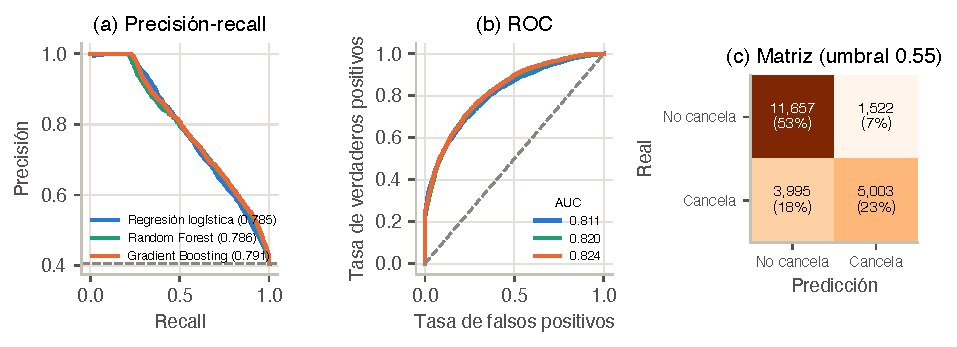
\includegraphics[width=0.85\textwidth]{fig13_prueba.pdf}
\caption{Prueba temporal: curvas precisión-\emph{recall} (a) y ROC (b) de los tres modelos, y
matriz de confusión del modelo final (c).}\label{fig:prueba}
\end{figure*}

La caída frente a la validación (0.873 a 0.784) se explica por la deriva que ya habíamos visto en
la Entrega 1. El modelo sigue ordenando las reservaciones de forma razonable, pero sus
probabilidades quedan cortas: marca como cancelación al 24\,\% de las reservaciones cuando en
realidad cancela el 41\,\%. Con el umbral de 0.72 la precisión es alta (0.81) y el \emph{recall}
baja a 0.48. Por hotel, el problema se concentra en el resort: su \emph{recall} es 0.28, contra
0.56 en el urbano, y su PR-AUC es 0.71 contra 0.81. En prueba los tres modelos quedan
prácticamente empatados en PR-AUC (0.784 a 0.787). La logística, menos flexible, resiste mejor el
cambio de distribución y con umbral 0.5 obtiene el mejor F1 (0.68).

En términos del negocio, el modelo anticipa 4,313 de las 8,998 cancelaciones del periodo con 1,023
falsas alarmas. Eso equivale a 2.23 de los 4.99 millones de ingreso en riesgo (45\,\%) y a 15,879
habitaciones-noche. Con $\kappa = 1.5$, el costo de las cancelaciones baja 28\,\% frente a no usar el
modelo; en validación esperábamos 47\,\%, y la diferencia es otra vez efecto de la deriva.

\subsection{Factores que más pesan}

Usamos dos métodos (Tabla~\ref{tab:top10}). La importancia por permutación mide cuánto cae la
PR-AUC de prueba al desordenar una variable. Los valores SHAP~\cite{lundberg2017,lundberg2020}
reparten cada predicción, en \emph{log-odds}, entre las variables; en nuestro caso la suma
reconstruye la salida del modelo con un error de $10^{-13}$. Para compararlos, sumamos las columnas
\emph{one-hot} de vuelta a su variable original.

Los dos métodos coinciden en las primeras posiciones: tipo de depósito, solicitudes especiales,
anticipación, agencia, tipo de cliente y segmento de mercado, lo mismo que anticipaba el análisis
exploratorio. La Fig.~\ref{fig:shap} agrega la dirección del efecto: \emph{Non Refund} empuja con
fuerza hacia la cancelación, cada solicitud especial empuja en contra y la anticipación larga
aumenta el riesgo. Las diferencias entre métodos vienen de variables correlacionadas. La tasa de
cancelación previa es 6.ª en SHAP y 20.ª en permutación porque \texttt{previous\_cancellations}
lleva casi la misma información, y al permutar una el modelo se apoya en la otra. La frecuencia de
la agencia, la variable nueva de esta entrega, queda 4.ª en SHAP.

\begin{table}[t]
\centering
\caption{Diez variables más importantes (SHAP) y su posición por permutación}\label{tab:top10}
\begin{tabular}{clcc}
\toprule
\# & Variable & $|$SHAP$|$ medio & Permutación \\
\midrule
\tabla{top10}
\bottomrule
\end{tabular}
\end{table}

\begin{figure}[t]
\centering
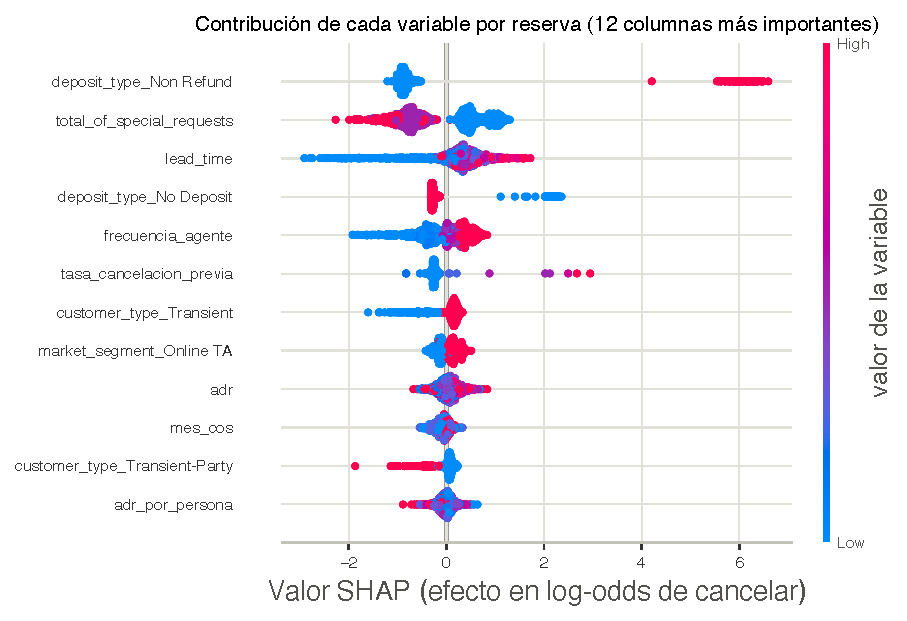
\includegraphics[width=\columnwidth]{fig16_shap.pdf}
\caption{Valores SHAP de 2,000 reservaciones de prueba. Cada punto es una reservación; el color es
el valor de la variable.}\label{fig:shap}
\end{figure}

\section{Empaquetado y despliegue preliminar}\label{sec:despliegue}

Aunque el despliegue corresponde a la última fase, empaquetamos el modelo para probarlo de punta a
punta. El \texttt{Pipeline} completo, el umbral y los metadatos (métricas, hiperparámetros,
variables y limitaciones) se guardan en un archivo de 3~MB. Un servidor del \emph{Model Context
Protocol}~\cite{mcp}, desplegado en Render, expone tres herramientas: predecir una reservación,
predecir un lote de hasta 500 y describir el modelo. Así, un asistente como Claude puede responder
preguntas como ``¿qué probabilidad hay de que se cancele esta reservación?'' usando las mismas
funciones de limpieza e ingeniería de características que el entrenamiento.

\section{Cumplimiento de objetivos}\label{sec:objetivos}

La Tabla~\ref{tab:objetivos} compara lo que planteamos en la Entrega 1 con lo que obtuvimos.

\begin{table*}[t]
\centering
\caption{Objetivos específicos de la Entrega 1 y resultado}\label{tab:objetivos}
\begin{tabular}{lL{6.2cm}L{8.3cm}}
\toprule
Objetivo & Planteamiento & Resultado \\
\midrule
OE1 & Clasificar variables y medir el efecto de las sospechosas & 3 excluidas; las 3 sospechosas suben la PR-AUC 5.3 puntos y se dejan fuera. Cumplido. \\
OE2 & \texttt{Pipeline} reproducible con al menos 5 variables derivadas & \texttt{Pipeline} ajustado solo en entrenamiento; 14 variables nuevas. Cumplido. \\
OE3 & Tres algoritmos, CV de 5 pliegues y búsqueda de hiperparámetros & Logística (NumPy), bosque y \emph{gradient boosting}; CV agrupada; rejilla y búsqueda aleatoria. Cumplido. \\
OE4 & ROC-AUC $\geq$ 0.85 y PR-AUC $\geq$ 0.75 en prueba; umbral por costos & PR-AUC 0.784 (cumple), ROC-AUC 0.816 (no cumple); umbral por costo esperado con sensibilidad a $\kappa$. Parcial. \\
OE5 & Diez factores con permutación y SHAP; traducción al negocio & Ambos métodos reportados; 45\,\% del ingreso en riesgo anticipado. Cumplido. \\
\bottomrule
\end{tabular}
\end{table*}

\section{Conclusiones y siguientes pasos}

La preparación quedó completa y reproducible, y la mayoría de los riesgos que identificamos en la
Entrega 1 se confirmaron: las variables sospechosas sí inflan el desempeño y la deriva temporal sí
pesa en la prueba. El \emph{gradient boosting} es el mejor modelo en validación, pero en datos de
2017 los tres modelos quedan casi empatados, y la meta de ROC-AUC no se alcanzó por el cambio en el
resort.

Para la fase de evaluación y despliegue nos quedan tres tareas. La primera es reentrenar con
ventanas recientes y recalibrar las probabilidades, para medir si la ROC-AUC se recupera. La
segunda es fijar $\kappa$ con costos reales de reubicación y revisar el umbral cada trimestre. La
tercera es monitorear en operación la tasa de cancelación predicha contra la real, que es la
señal más directa de que el modelo se está quedando atrás.

\begin{thebibliography}{99}
\bibitem{antonio2017} N. Antonio, A. de Almeida y L. Nunes, ``Predicting hotel booking cancellations to decrease uncertainty and increase revenue,'' \emph{Tourism \& Management Studies}, vol. 13, no. 2, pp. 25--39, 2017, doi: 10.18089/tms.2017.13203.
\bibitem{pedregosa} F. Pedregosa \emph{et al.}, ``Scikit-learn: Machine learning in Python,'' \emph{J. Mach. Learn. Res.}, vol. 12, pp. 2825--2830, 2011.
\bibitem{kaufman} S. Kaufman, S. Rosset y C. Perlich, ``Leakage in data mining: Formulation, detection, and avoidance,'' en \emph{Proc. 17th ACM SIGKDD Int. Conf. Knowl. Discov. Data Min.}, 2011, pp. 556--563, doi: 10.1145/2020408.2020496.
\bibitem{chapman} P. Chapman \emph{et al.}, \emph{CRISP-DM 1.0: Step-by-step data mining guide}. SPSS, 2000.
\bibitem{antonio2019} N. Antonio, A. de Almeida y L. Nunes, ``Hotel booking demand datasets,'' \emph{Data in Brief}, vol. 22, pp. 41--49, 2019, doi: 10.1016/j.dib.2018.11.126.
\bibitem{tidytuesday} R for Data Science Online Learning Community, ``Hotels,'' TidyTuesday, semana 2020-02-11, GitHub, 2020. [En línea]. Disponible: \url{https://github.com/rfordatascience/tidytuesday/tree/master/data/2020/2020-02-11}
\bibitem{saito} T. Saito y M. Rehmsmeier, ``The precision-recall plot is more informative than the ROC plot when evaluating binary classifiers on imbalanced datasets,'' \emph{PLOS ONE}, vol. 10, no. 3, art. e0118432, 2015, doi: 10.1371/journal.pone.0118432.
\bibitem{breiman} L. Breiman, ``Random forests,'' \emph{Machine Learning}, vol. 45, no. 1, pp. 5--32, 2001, doi: 10.1023/A:1010933404324.
\bibitem{friedman} J. H. Friedman, ``Greedy function approximation: A gradient boosting machine,'' \emph{Ann. Statist.}, vol. 29, no. 5, pp. 1189--1232, 2001, doi: 10.1214/aos/1013203451.
\bibitem{lightgbm} G. Ke \emph{et al.}, ``LightGBM: A highly efficient gradient boosting decision tree,'' en \emph{Advances in Neural Information Processing Systems 30}, 2017, pp. 3146--3154.
\bibitem{bergstra} J. Bergstra y Y. Bengio, ``Random search for hyper-parameter optimization,'' \emph{J. Mach. Learn. Res.}, vol. 13, pp. 281--305, 2012.
\bibitem{elkan} C. Elkan, ``The foundations of cost-sensitive learning,'' en \emph{Proc. 17th Int. Joint Conf. Artif. Intell.}, 2001, pp. 973--978.
\bibitem{lundberg2017} S. M. Lundberg y S.-I. Lee, ``A unified approach to interpreting model predictions,'' en \emph{Advances in Neural Information Processing Systems 30}, 2017, pp. 4765--4774.
\bibitem{lundberg2020} S. M. Lundberg \emph{et al.}, ``From local explanations to global understanding with explainable AI for trees,'' \emph{Nature Machine Intelligence}, vol. 2, pp. 56--67, 2020, doi: 10.1038/s42256-019-0138-9.
\bibitem{mcp} Anthropic, ``Model Context Protocol,'' especificación, 2024. [En línea]. Disponible: \url{https://modelcontextprotocol.io}
\bibitem{repo} H. Á. Plata Durán y D. Hernández Ortiz, ``Predicción de cancelaciones de reservas hoteleras,'' repositorio en GitHub, 2026. [En línea]. Disponible: \url{https://github.com/BetoPD/prediccion-cancelaciones-hoteles}
\end{thebibliography}

\end{document}
